\documentclass[12pt, letterpaper]{article}

\usepackage{amsmath, amssymb, amsthm, mathrsfs}
\usepackage{geometry}
\usepackage{tikz}
\usepackage{titlesec}
\usepackage{enumitem}
\usepackage{hyperref}
\usepackage{setspace}
\usepackage{xcolor}
\usepackage{mathtools}
\usepackage{tikz-cd}
\usepackage{booktabs}
\usepackage{longtable}
\usepackage{caption}

\hyphenpenalty=10000
\exhyphenpenalty=10000
\pretolerance=10000
\sloppy

\geometry{
    top=1.25in,
    bottom=1.25in,
    left=1.5in,
    right=1.5in
}

\doublespacing

\theoremstyle{definition}
\newtheorem{definition}{Definition}[section]
\newtheorem{remark}[definition]{Remark}
\newtheorem{example}[definition]{Example}

\theoremstyle{plain}
\newtheorem{theorem}{Theorem}[section]
\newtheorem{lemma}[theorem]{Lemma}
\newtheorem{proposition}[theorem]{Proposition}
\newtheorem{corollary}[theorem]{Corollary}
\newtheorem{conjecture}[theorem]{Conjecture}
\newtheorem*{theorem*}{Theorem}
\newtheorem*{remark*}{Remark}
\newtheorem{mainthm}{Theorem}
\renewcommand{\themainthm}{\Alph{mainthm}}
\newtheorem{maincor}[mainthm]{Corollary}

\title{\vspace{-2cm}\Large\textbf{How Few Heat Invariants Determine a Hyperbolic Triangular Pillow}}

\date{}

\begin{document}

\maketitle
\thispagestyle{empty}

\begin{abstract}
    \noindent We study the inverse spectral geometry of hyperbolic triangular pillows ,  spheres carrying three cone points, the orbifold quotients of hyperbolic triangle groups ,  and determine exactly how much of the singular geometry is fixed by the leading coefficients of the heat trace. The two leading heat coefficients determine such a pillow, among all of them, precisely when its cone orders satisfy $p+q+r\le 17$. This is a sharp structural rigidity threshold: we prove it not by enumeration but by showing that the reciprocal-sum data of the pillows, stratified by least cone order, occupy monotone intervals that stay disjoint through sum $17$ and first touch at sum $18$, where the rigidity breaks. At that first touch the non-isometric pillows $\mathcal{O}(2,8,8)$ and $\mathcal{O}(3,3,12)$ share their two leading heat coefficients ,  the minimal two-coefficient spectral degeneracy, realized as the meeting of the balanced boundary of one stratum and the concentrated boundary of the next. The threshold at $17$ and its first degeneracy at $18$ are the sharp base cases of a Diophantine problem we then take up in its own right: the asymptotic density and frequency of two-coefficient degeneracies at large cone-order sum, each such degeneracy being a pair of three-term Egyptian-fraction representations of a common value with equal denominator sum. We prove that degeneracies recur at every multiple of the base sum $18$ via an exact scaling law, giving the unconditional lower bound $\mathcal N(S)\ge\lfloor S/18\rfloor$ for the cumulative count; exact-arithmetic enumeration through $S=600$ shows this undercounts the true growth substantially, with $\mathcal N(S)$ tracking $c\,S^2$ for $c\approx0.0085$--$0.0093$, and we set out the matching birthday-type heuristic as a precise conjecture. Two heat coefficients detect the area and the total cone order but not the distribution of cone angles; the first three always determine the pillow up to isometry, the three invariant functions forming local coordinates on cone-order space away from its diagonals, with the third ,  a constant-curvature cone invariant of Dryden--Gordon--Greenwald--Webb, Schueth, and U\c{c}ar ,  supplying the missing symmetric function of the orders. All numerical assertions are verified in exact rational arithmetic.
\end{abstract}

\vspace{0.8cm}
\noindent\textbf{Keywords:} Inverse spectral geometry; heat-trace coefficients; Riemannian orbifolds; cone singularities and singular strata; hyperbolic triangle orbifolds; spectral determinacy and non-determinacy; spectral degeneracies; Egyptian fractions.

\smallskip
\noindent\textbf{2020 MSC:} 58J53, 58J50, 35K08, 11D45, 11D68.

\newpage
\tableofcontents
\newpage


\section{Introduction}
\label{sec:intro}

Inverse spectral geometry asks how much of the geometry of a space is encoded in the spectrum of its Laplace--Beltrami operator~\cite{kac1966}. For singular spaces the question sharpens: the heat trace carries not only smooth Riemannian data but also the geometry of the singular set, and one may ask precisely which singular features it records. We study this for a concrete family of hyperbolic cone orbifolds in the most quantitative form available ,  not merely \emph{whether} the spectrum determines the geometry, but \emph{how many} of the leading heat-trace coefficients are needed and \emph{what singular geometry each one encodes}.

A \emph{hyperbolic triangular pillow} $\mathcal{O}(p,q,r)$ is the sphere carrying three cone points of orders $2\le p\le q\le r$ with $\tfrac1p+\tfrac1q+\tfrac1r<1$. It is the quotient orbifold of a hyperbolic triangle group, equivalently the metric double of a hyperbolic triangle with angles $\pi/p,\pi/q,\pi/r$: two identical copies of the triangle glued along their boundary (Figure~\ref{fig:pillow}).

\begin{figure}[h!]
    \centering
    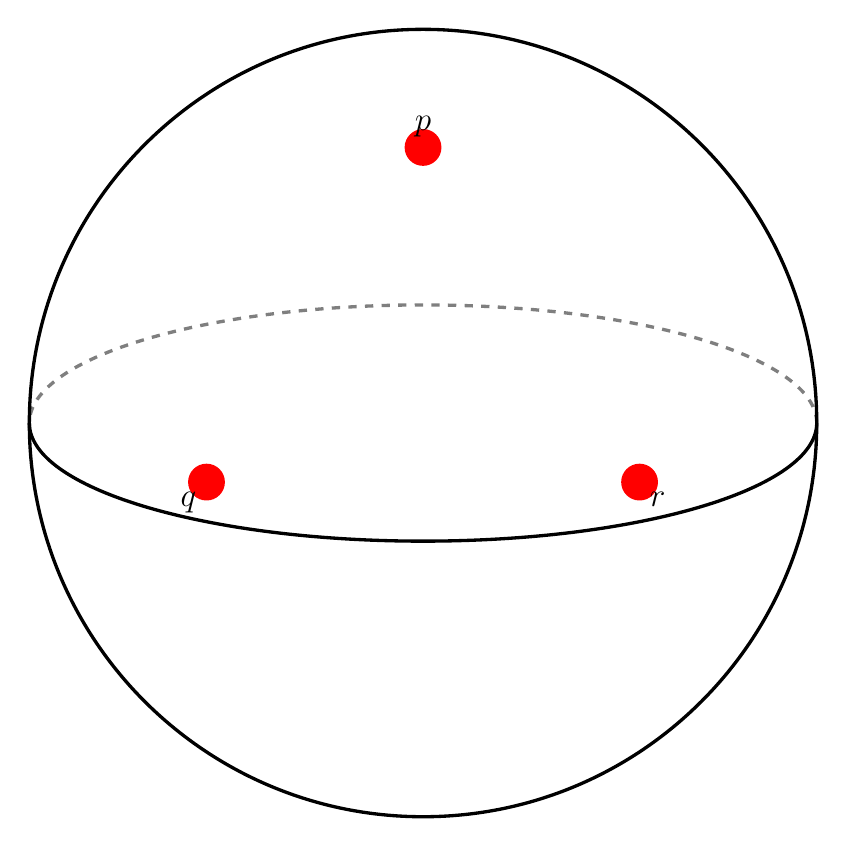
\begin{tikzpicture}[scale=2.5, thick]
        \draw[line width=1.2pt] (0,0) circle (2cm);
        \draw[line width=1.2pt] (-2,0) arc (180:360:2 and 0.6);
        \draw[dashed, opacity=0.5, line width=1.2pt] (2,0) arc (0:180:2 and 0.6);

        \filldraw[red] (0, 1.4) circle (2.5pt) node[above, text=black, font=\large] {$p$};
        \filldraw[red] (-1.1, -0.3) circle (2.5pt) node[below left, text=black, font=\large] {$q$};
        \filldraw[red] (1.1, -0.3) circle (2.5pt) node[below right, text=black, font=\large] {$r$};
    \end{tikzpicture}
    \caption{The pillow $\mathcal{O}(p,q,r)$: the double of a hyperbolic triangle with angles $\pi/p,\pi/q,\pi/r$, a sphere with three cone points of orders $p,q,r$.}
    \label{fig:pillow}
\end{figure}

By the Gauss--Bonnet theorem the area is
\begin{equation}
    \operatorname{Area}(\mathcal{O}) = 2\pi \left( 1 - \Big( \tfrac{1}{p} + \tfrac{1}{q} + \tfrac{1}{r} \Big) \right),
    \label{eq:area}
\end{equation}
and hyperbolicity is the condition $\tfrac1p+\tfrac1q+\tfrac1r<1$.

The leading coefficients of the heat trace $\operatorname{tr}e^{-t\Delta}$ are geometric invariants of $\mathcal{O}(p,q,r)$, and our results describe, coefficient by coefficient, how much of its singular geometry they determine. The \emph{analytic} input is classical: the orbifold heat expansion of Donnelly and Dryden--Gordon--Greenwald--Webb~\cite{donnelly1976, dggw2008} attaches to each cone point an explicit contribution to every coefficient, so that the leading coefficients become symmetric functions of the cone orders. The question we answer is \emph{geometric}: how far these low-order symmetric aggregates go toward pinning down the singular stratum ,  the cone points together with their orders. The dividing line is \emph{arithmetic}, governed by when two triples of orders share prescribed symmetric functions; where the answer is finite and exact we certify it by a bounded computation in exact rational arithmetic, rather than leave it asymptotic.

Our main results are the following. Throughout, $K(F)$ denotes the least number of leading heat coefficients that distinguish a pillow $F$ from every other hyperbolic triangular pillow, and a pair of non-isometric pillows sharing their first two heat coefficients is a \emph{two-coefficient spectral degeneracy}, or \emph{collision} ,  the two terms are used interchangeably.

\begin{mainthm}[Finite-coefficient determinacy threshold]\label{thmA}
Let $F=\mathcal{O}(p,q,r)$ be a hyperbolic triangular pillow. If $p+q+r\le17$, then $F$ is determined among all hyperbolic triangular pillows by its first two heat coefficients, so $K(F)\le2$. The bound $17$ is sharp: two coefficients no longer determine every pillow once the cone-order sum reaches $18$ (Theorem~\ref{thmB}).
\end{mainthm}

\begin{mainthm}[Minimal two-coefficient degeneracy]\label{thmB}
The non-isometric pillows $\mathcal{O}(2,8,8)$ and $\mathcal{O}(3,3,12)$ have identical first two heat coefficients. Among all two-coefficient degeneracies this pair has the smallest cone-order sum, $p+q+r=18$; it is the unique degeneracy at that sum, and none occurs for $p+q+r\le17$.
\end{mainthm}

\begin{mainthm}[Three-coefficient determinacy of the cone-order multiset]\label{thmC}
The first three heat coefficients determine a hyperbolic triangular pillow up to isometry ,  equivalently, they determine its singular set together with the cone order at each singular point. Thus $K(F)\le3$ for every such pillow, and $K(F)=3$ for the collision pair $\mathcal{O}(2,8,8),\mathcal{O}(3,3,12)$ of Theorem~\ref{thmB}.
\end{mainthm}

\begin{maincor}[What the heat coefficients detect]\label{corD}
For $\mathcal{O}(p,q,r)$ write $R=\sum_i m_i^{-1}$ and $S_1=\sum_i m_i$. The first heat coefficient detects the area, equivalently $R$; the first two factor through the pair $(R,S_1)$ ,  the area and the total cone order ,  so that two-coefficient determinacy is exactly injectivity of the map $(p,q,r)\mapsto(R,S_1)$; the first three additionally detect $\sum_i m_i^3$, hence the individual cone orders. Consequently the two leading coefficients resolve the full singular stratum for every pillow with $p+q+r\le17$, and this range is sharp: the first failure occurs at $p+q+r=18$, for the pair of Theorem~\ref{thmB}. The larger-sum pillows for which two coefficients fail to suffice are enumerated, and their density studied, in Section~\ref{sec:density}.
\end{maincor}

Together these describe a single geometric hierarchy: the first heat coefficient records the area, the first two additionally record the total cone order, and the third completes the singular stratum, with the threshold of Theorem~\ref{thmA} marking exactly where two coefficients cease to suffice. Theorem~\ref{thmA} and its sharp failure in Theorem~\ref{thmB} are proved in Section~\ref{sec:threshold} through the interval-separation mechanism; Theorem~\ref{thmC} and Corollary~\ref{corD} are proved in Section~\ref{sec:geometry}, where we read the collision as a statement about singular geometry. The threshold at $17$ is not an endpoint but a point of departure: at sum $18$ the two-coefficient map first fails to be injective, and how often ,  and how densely ,  it fails as the cone-order sum grows is an asymptotic Diophantine problem in its own right, which we formulate and study in Section~\ref{sec:density}. The sum-$18$ degeneracy is its sharp base case.

\subsection{Related work}
\label{sec:related}

\emph{Reading geometry from finitely many heat invariants.} That a few leading heat-trace coefficients encode geometric data goes back to Kac~\cite{kac1966} and McKean--Singer~\cite{mckeansinger1967}, with the broader inverse-spectral program surveyed by Datchev--Hezari~\cite{datchevhezari2013}. Determinacy by a \emph{finite} amount of spectral data is known in several concrete families: Grieser--Maronna show a Euclidean triangle is determined by three invariants~\cite{griesermaronna2013}; Lu--Rowlett show the regular $n$-gon is determined among convex $n$-gons by finitely many eigenvalues~\cite{lurowlett2015}; and Hezari--Zelditch prove spectral uniqueness of nearly circular ellipses~\cite{hezarizelditch2022}. Sharpness cuts both ways: G\'omez-Serrano--Orriols show three \emph{eigenvalues} do not determine a triangle~\cite{gomezserrano2020}, so both the choice of invariant and the exact count matter.

\emph{Isospectral constructions and the limits of hearing.} Non-isometric objects sharing the spectrum arise from Sunada's covering method~\cite{sunada1985} and the planar drums of Gordon--Webb--Wolpert~\cite{gww1992}. For orbifolds, Shams--Stanhope--Webb show one cannot hear the isotropy type~\cite{ssw2006}, Rossetti--Schueth--Weilandt construct isospectral orbifolds with different maximal isotropy orders~\cite{rsw2008}, and Bari--Hunsicker analyse how few heat coefficients suffice for orbifold lens spaces~\cite{barihunsicker2017}.

\emph{Orbifold heat invariants.} The heat-trace asymptotics we use are those of Donnelly~\cite{donnelly1976} and Dryden--Gordon--Greenwald--Webb~\cite{dggw2008}; recent positive results in the orbifold setting include Proctor--Stanhope~\cite{proctorstanhope2009}, Richardson--Stanhope on local orientability~\cite{richardsonstanhope2019}, and Gittins et al.\ on whether spectra distinguish orbifolds from manifolds~\cite{gittinsetal2024}.

\emph{Cone and corner contributions.} The third coefficient we need is governed by the constant-curvature cone coefficients of Schueth~\cite{schueth2019, schueth2025} and U\c{c}ar~\cite{ucar2017}, within the broader analytic theory of heat traces on conic and polygonal domains developed by Suleymanova~\cite{suleymanova2017}, Nursultanov--Rowlett--Sher~\cite{nrs2024}, and Looi--Sher~\cite{looisher2025}.

\emph{Hyperbolic orbisurfaces and triangle groups.} In the hyperbolic setting, Dryden--Strohmaier prove a Huber theorem relating the Laplace and length spectra of orbisurfaces~\cite{drydenstrohmaier2009}, Doyle--Rossetti show isospectral hyperbolic surfaces have matching geodesics~\cite{doylerossetti2008}, and Harmer computes the spectra of the spherical and Euclidean triangle groups~\cite{harmer2008}; the underlying triangle-orbifold geometry is standard~\cite{scott1983, buser1992}. Closest to the present work, U\c{c}ar~\cite{ucar2017} proves that the \emph{full} spectrum determines the cone-order multiset of an orientable constant-curvature orbisurface ,  the qualitative statement we sharpen to an exact finite coefficient count.

\subsection{Conventions}
\label{sec:conventions}

We use the orbifold heat-trace expansion of Dryden--Gordon--Greenwald--Webb~\cite{dggw2008}. With the smooth principal-stratum series carrying the $(4\pi t)^{-1}$ prefactor and each cone point $C$ of order $m$ contributing $b_\ell(C)$ at order $t^{\ell}$, the degree-zero (constant) coefficient of $\mathcal{O}(p,q,r)$ is
\begin{equation}
    a_0 \;=\; \frac{\chi(\mathcal{O})}{6} \;+\; \sum_{i}\frac{m_i^2-1}{12\,m_i},
    \label{eq:a0conv}
\end{equation}
where $\chi(\mathcal{O}) = 2 - \sum_i(1-\tfrac1{m_i}) = R-1$ is the orbifold Euler characteristic, $R:=\sum_i \tfrac1{m_i}$, and the normalization is the $1/(4\pi)$ of~\cite{dggw2008} (no separate Euler factor). As a fixed reference point, the spherical triple $(2,3,5)$ gives cone sum $\tfrac18+\tfrac29+\tfrac25=\tfrac{269}{360}$ and, with the smooth term $\chi/6=\tfrac1{180}$, total $a_0=\tfrac{271}{360}$.

\subsection{Locating the novelty}
\label{sec:novelty}

We state plainly what is new and what is not.

\emph{(a) Prior art.} The orbifold heat-trace expansion and the cone contribution $\tfrac{m^2-1}{12m}$ are due to~\cite{donnelly1976, dggw2008}; the higher constant-curvature cone coefficients are those of~\cite{dggw2008, schueth2019, ucar2017}. Crucially, U\c{c}ar~\cite{ucar2017} already proves that the \emph{full} spectrum determines the cone-order multiset of an orientable constant-curvature orbisurface, and~\cite{dggw2008, ucar2017} record the known spherical near-collisions. All of this determinacy is \emph{asymptotic or full-spectrum and qualitative}; none of it counts coefficients or exhibits a sharp finite boundary. We do not reprove any of it.

\emph{(b) Our contribution.} We refine this qualitative, full-spectrum picture into an exact finite-coefficient one. Theorems~\ref{thmA}--\ref{thmC} and Corollary~\ref{corD} determine, for a hyperbolic triangular pillow, how many leading heat coefficients are needed and what singular geometry each encodes: a sharp threshold below which two coefficients suffice (Theorem~\ref{thmA}), an explicit minimal pair they fail to separate (Theorem~\ref{thmB}), and the full singular stratum recovered by three (Theorem~\ref{thmC}, Corollary~\ref{corD}). To our knowledge this is the first exact finite-coefficient determinacy threshold, with an explicit minimal degeneracy, for a family of hyperbolic cone orbifolds. The two supporting steps are classical and we treat them as such ,  the cone identity $\sum_j\csc^2(j\pi/m)=\tfrac{m^2-1}{3}$ and the Newton--Vieta recovery of $(p,q,r)$ from three symmetric functions; the sharpness and minimality are then proved through the monotone interval structure of Theorem~\ref{thm:separation}, which forces the threshold from the geometry of the two-coefficient map and reduces it to a short list of explicit endpoint inequalities rather than an unbounded search. Beyond these base cases we recast two-coefficient non-determinacy as an asymptotic Diophantine problem ,  the density and frequency of spectral degeneracies at large cone-order sum ,  and study its growth in Section~\ref{sec:density}, where we prove an exact scaling law forcing infinitely many degeneracies and giving an unconditional linear lower bound, and set out a numerically-supported quadratic growth conjecture.

\emph{(c) Load-bearing only.} We introduce no machinery that is not used in a proof: the third heat coefficient is used as computed in~\cite{dggw2008, schueth2019, ucar2017}, not rederived, and the constrained minimizer of Section~\ref{sec:geometry} is the Cauchy--Schwarz inequality, not a spectral-rigidity statement. The nearest exact hyperbolic-spectrum precedent is Doyle--Rossetti~\cite{doylerossetti2008}, whose concern ,  matching length spectra ,  is orthogonal to our finite-coefficient count.

\subsection{Scope and limitations}
\label{sec:scope}

We delimit the result precisely. (i) It concerns hyperbolic \emph{triangular} pillows ,  three cone points on a sphere; the $n$-cone generalization is discussed in Remark~\ref{rem:ncone} and established here only for $n=3$. (ii) The hyperbolic third coefficient is used as established in~\cite{dggw2008, schueth2019, ucar2017}; we verify its constant-curvature specialization and its effect on determinacy, but do not advance the cone-coefficient theory itself, and the recent curved-cone results of~\cite{schueth2025} do \emph{not} apply, since a constant-curvature orbifold cone has no curvature blow-up at the tip. (iii) The threshold and the minimal degeneracy are proved through the interval-separation mechanism (Theorem~\ref{thm:separation}), which reduces them to finitely many explicit rational inequalities between stratum endpoints ,  three adjacent-pair comparisons for $S_1\le17$ and four endpoint comparisons at $S_1=18$; this is a structural argument, not an exhaustive search, and the full enumeration in Appendix~\ref{sec:appendix} (Table~\ref{tab:enum}) is independent corroboration. (iv) The two-coefficient theory has $K(F)\le3$ unconditionally (Theorem~\ref{thmC}); the density and frequency of two-coefficient degeneracies at large cone-order sum ,  and hence the exact set of pillows with $K(F)=3$ ,  is the subject of Section~\ref{sec:density}, whose base case at sum $18$ is settled unconditionally, whose infinitude and linear-order growth are proved via an exact scaling law, and whose conjectured quadratic-order growth is supported by exact-arithmetic enumeration through sum $600$.

\newpage
\section{Heat coefficients of a hyperbolic triangular pillow}
\label{sec:core}

We assemble the three leading heat coefficients as symmetric functions of the cone orders. Each cone point contributes to every coefficient through the orbifold expansion of~\cite{dggw2008}; we make the first three contributions explicit and record how they invert to the orders. The computations are classical and we keep them brief.

\subsection{The heat expansion}
\label{sec:heatexp}

On a closed hyperbolic $2$-orbifold $\mathcal{O}$ the heat trace has the small-time asymptotic expansion of Minakshisundaram--Pleijel type~\cite{mckeansinger1967}, refined to the orbifold stratification by Donnelly and Dryden--Gordon--Greenwald--Webb~\cite{donnelly1976, dggw2008}. It splits along the strata:
\[
    \operatorname{tr}e^{-t\Delta}\ \sim\ \underbrace{(4\pi t)^{-1}\sum_{\ell\ge0} a^{\mathrm{sm}}_\ell\, t^{\ell}}_{\text{principal (smooth) stratum}}\ +\ \sum_{\text{cone points }C}\ \underbrace{\sum_{\ell\ge0} b_\ell(C)\, t^{\ell}}_{\text{singular stratum}},
\]
where each $a^{\mathrm{sm}}_\ell$ is the integral over $\mathcal{O}$ of a universal polynomial in the curvature and its covariant derivatives, and each cone point $C$ (a zero-dimensional singular stratum) contributes a series $b_\ell(C)$ carrying no $(4\pi t)^{-1}$ prefactor. Because the cones have constant curvature the expansion contains only integer powers of $t$: the half-integer and logarithmic terms that arise for genuinely curved conical singularities~\cite{schueth2025, suleymanova2017, nrs2024} are absent, as a constant-curvature orbifold cone has no curvature blow-up at the tip. The three invariants of this paper are the coefficients of $t^{-1}$, $t^{0}$, and $t^{1}$. At constant curvature each smooth term $a^{\mathrm{sm}}_\ell$ is a fixed multiple of $\operatorname{Area}(\mathcal{O})$, hence a function of $R$ alone; the geometric content beyond the area therefore lives entirely in the cone-point sums $\sum_i b_\ell(C_i)$, which we compute in the next two subsections.

\subsection{The cone contribution}
\label{sec:cone}

\begin{lemma}[Cotangent sum]\label{lem:cot}
For every integer $m\ge2$, $\ \displaystyle\sum_{j=1}^{m-1}\cot^2\!\Big(\tfrac{j\pi}{m}\Big)=\tfrac{(m-1)(m-2)}{3}$.
\end{lemma}

\begin{proof}
Let $P(z)=(z+1)^m-(z-1)^m$. By the binomial theorem $P(z)=\sum_k\binom{m}{k}[1-(-1)^{m-k}]z^k$, so only powers $z^k$ with $m-k$ odd survive, each with coefficient $2\binom{m}{k}$; the top three coefficients are $[z^{m-1}]P=2m$, $[z^{m-2}]P=0$, $[z^{m-3}]P=2\binom{m}{3}$, and $\deg P=m-1$. For $z\ne1$, $P(z)=0$ iff $\big(\tfrac{z+1}{z-1}\big)^m=1$; the M\"obius map $z\mapsto\tfrac{z+1}{z-1}$ is injective and omits the value $1$, so the roots are $z_j=-i\cot(j\pi/m)$, $j=1,\dots,m-1$, and these $m-1$ distinct numbers are all of them. By Vieta, $\sum_j z_j=0$ and $\sum_{i<j}z_iz_j=\binom{m}{3}/m=(m-1)(m-2)/6$, so $\sum_j z_j^2=-\tfrac{(m-1)(m-2)}{3}$. Since $z_j^2=-\cot^2(j\pi/m)$, the claim follows.
\end{proof}

\begin{proposition}[Cosecant sum]\label{prop:csc}
For every integer $m\ge2$, $\ \displaystyle\sum_{j=1}^{m-1}\csc^2\!\Big(\tfrac{j\pi}{m}\Big)=\tfrac{m^2-1}{3}$.
\end{proposition}

\begin{proof}
By $\csc^2=1+\cot^2$ and Lemma~\ref{lem:cot}, $\sum_j\csc^2(j\pi/m)=(m-1)+\tfrac{(m-1)(m-2)}{3}=\tfrac{(m-1)(m+1)}{3}=\tfrac{m^2-1}{3}$.
\end{proof}

In the convention of~\cite{dggw2008} a rotation of order $m$ through angle $2\pi j/m$ contributes $b_0(\gamma^j)=\tfrac14\csc^2(j\pi/m)$ to its fixed-point stratum, and the stratum term is divided by the isotropy order $m$.

\begin{definition}\label{def:cone}
The \emph{cone contribution} of a cone point of order $m\ge2$ is
$\ \operatorname{cone}(m):=\tfrac{1}{4m}\sum_{j=1}^{m-1}\csc^2(j\pi/m)$.
\end{definition}

\begin{corollary}\label{cor:conevals}
$\operatorname{cone}(m)=\dfrac{m^2-1}{12m}=\tfrac1{12}\big(m-\tfrac1m\big)$; in particular $\operatorname{cone}(2)=\tfrac18$, $\operatorname{cone}(3)=\tfrac29$, $\operatorname{cone}(5)=\tfrac25$.
\end{corollary}

\begin{proof}
Substitute Proposition~\ref{prop:csc} into Definition~\ref{def:cone}: $\operatorname{cone}(m)=\tfrac{1}{4m}\cdot\tfrac{m^2-1}{3}=\tfrac{m^2-1}{12m}$.
\end{proof}

The prefactor is $\tfrac1{4m}$ (the $\tfrac14$ weight of each rotation, times the $\tfrac1m$ isotropy division), not a flat $\tfrac1{12}$; the contribution is curvature-independent at this order, so it is the same for flat and hyperbolic cones.

\subsection{Three invariants and the corrected inversion}
\label{sec:inversion}

Write the elementary symmetric functions $e_1=p+q+r=S_1$, $e_2=pq+qr+rp$, $e_3=pqr$, so $R=e_2/e_3$. The heat expansion supplies, in order:

\begin{enumerate}[label=(\roman*)]
\item \textbf{Area.} By~\eqref{eq:area} the first coefficient determines $R=\tfrac1p+\tfrac1q+\tfrac1r=e_2/e_3$.
\item \textbf{Zeroth coefficient.} By~\eqref{eq:a0conv} and Corollary~\ref{cor:conevals}, using $\sum_i\operatorname{cone}(m_i)=\tfrac1{12}(S_1-R)$ and $\chi/6=(R-1)/6$,
\begin{equation}
    a_0=\frac{S_1+R-2}{12}\qquad\Longleftrightarrow\qquad \boxed{\,S_1=12\,a_0+2-R\,}.
    \label{eq:s1inv}
\end{equation}
With $R$ known, \eqref{eq:s1inv} returns $S_1=e_1$.
\item \textbf{Third invariant.} The third coefficient supplies one further symmetric function $I_3$, independent of $(S_1,R)$; it is derived in Section~\ref{sec:a2}.
\end{enumerate}

\begin{remark}\label{rem:bugfix}
The constant $+2$ in~\eqref{eq:s1inv} is the smooth term $\chi(\mathcal{O})/6=(R-1)/6$ carried through the inversion. Treating the topological Euler characteristic of the underlying sphere as an additive constant instead would give $S_1=12(a_0-2)+R$, which already fails the reference triple: it returns a negative value for $(2,3,5)$, where $S_1=10$. We record the correct normalization to preclude this.
\end{remark}

\subsection{The hyperbolic third coefficient}
\label{sec:a2}

The three leading coefficients are those of $t^{-1}$ (area, giving $R$), $t^0$ (giving $S_1$), and $t^1$. For a cone of order $m$ and Gauss curvature $K$, the constant-curvature cone coefficient at order $t^1$ is\footnote{The expression~\eqref{eq:b1} is quoted from the constant-curvature cone/orbifold literature, not rederived here. It is the cone-point coefficient $a_1(\{\bar p\})$ of Schueth~\cite{schueth2019}, Remark~4.2 (there attributed to Dryden--Gordon--Greenwald--Webb~\cite{dggw2008}, §5.6), restated with the same attribution in~\cite{schueth2025}, and consistent with U\c{c}ar's constant-curvature form $b_\ell(C)=\kappa^\ell\tfrac1m p_\ell(m)$, $\deg p_\ell=2\ell+2$~\cite{ucar2017}. We use only the specialization $K=-1$. The normalization matches Section~\ref{sec:conventions}: the smooth series carries the $(4\pi t)^{-1}$ prefactor, while a cone point ,  a zero-dimensional stratum ,  contributes at order $t^\ell$ with no such prefactor (\cite{schueth2019}, Rem.~3.2) and with the $\tfrac1m$-average over the $m-1$ nontrivial rotations built in (\cite{schueth2019}, eq.~(17)).}
\begin{equation}
    b_1(C)=\Big[\tfrac1{360}\big(m^3-\tfrac1m\big)+\tfrac1{36}\big(m-\tfrac1m\big)\Big]K,
    \label{eq:b1}
\end{equation}
with $b_0(C)=\tfrac{m^2-1}{12m}$ as above. At constant negative curvature $K=-1$ the smooth part of the $t^1$ coefficient is a universal constant times $\operatorname{Area}(\mathcal{O})=2\pi(1-R)$, hence a function of the already-known $R$; the new content is $\sum_i b_1(C_i)$. Summing~\eqref{eq:b1} at $K=-1$,
\begin{equation}
    \sum_i b_1(C_i)\Big|_{K=-1}=-\tfrac1{360}\,P_3-\tfrac1{36}\,S_1+\tfrac{11}{360}\,R,\qquad P_3:=\sum_i m_i^3,
    \label{eq:a2red}
\end{equation}
using $\tfrac1{360}+\tfrac1{36}=\tfrac{11}{360}$. Thus, modulo $(S_1,R)$, the third invariant delivers the power sum $P_3=\sum m_i^3$. For the determinacy results only a weaker feature of~\eqref{eq:a2red} is needed: after subtracting the terms in $R$ and $S_1$ (both known from the first two coefficients), what remains is a \emph{nonzero} rational multiple of $P_3$ (here $-\tfrac1{360}$). The recovery of Proposition~\ref{prop:recovery} therefore depends on $b_1$ only through this nonvanishing $m^3$-coefficient, and is unaffected by the precise values of the lower-order terms of~\eqref{eq:b1}. This is not the flat-cone quantity $\sum m_i^{-3}$: a flat cone contributes nothing at this order ($b_1=0$ at $K=0$), so $\sum m_i^{-3}$ is not a hyperbolic heat invariant.

\begin{proposition}[Cauchy--Schwarz bound]\label{prop:cs}
For every hyperbolic triad, $S_1 R=(p+q+r)\big(\tfrac1p+\tfrac1q+\tfrac1r\big)\ge 9$, with equality iff $p=q=r$.
\end{proposition}

\begin{proof}
Cauchy--Schwarz (equivalently AM--HM) gives $9\le S_1 R$, with equality iff $m_1=m_2=m_3$.
\end{proof}

\begin{proposition}[Recovery from three symmetric functions]\label{prop:recovery}
The values $R=\sum_i m_i^{-1}$, $S_1=\sum_i m_i$, and $P_3=\sum_i m_i^{3}$ determine the multiset $\{p,q,r\}$; equivalently, the map sending a hyperbolic triangular pillow to its first three heat coefficients is injective.
\end{proposition}

\begin{proof}
By~\eqref{eq:a2red} the first three coefficients determine $(R,S_1,P_3)$. Write the elementary symmetric functions $e_1=S_1$, $e_2=pq+qr+rp$, $e_3=pqr$, so that $e_2=R\,e_3$. Newton's identity $P_3=e_1^3-3e_1e_2+3e_3=e_1^3+3e_3(1-e_1R)$ gives
\begin{equation}
    e_3=\frac{P_3-e_1^{3}}{\,3-3\,S_1 R\,},\qquad e_2=R\,e_3,
    \label{eq:e3}
\end{equation}
the denominator being nonzero by Proposition~\ref{prop:cs}. The cone orders are the roots of $z^3-e_1 z^2+e_2 z-e_3$.
\end{proof}

This Newton--Vieta inversion is a standard symmetric-function recovery. Its infinitesimal counterpart is immediate: the map $F=(S_1,R,P_3)$ has Jacobian determinant $\det DF=-3\,(p-q)(p-r)(q-r)(p+q)(p+r)(q+r)/(p^2q^2r^2)$, nonzero off the diagonals $p=q$, $p=r$, $q=r$, so the three invariants form a local coordinate system on each open ordered chamber $\{p<q<r\}$. This plays no role in the two-coefficient threshold of Section~\ref{sec:threshold}, which concerns the discrete map $\sigma=(S_1,R)$.

\newpage
\section{The determinacy threshold and the minimal degeneracy}
\label{sec:threshold}

We prove Theorems~\ref{thmA} and~\ref{thmB} without exhaustive tabulation. The two-coefficient invariant $R$, restricted to triads of a fixed cone-order sum and fixed least cone order, is strictly monotone (Lemma~\ref{lem:chamber}); the resulting \emph{strata} therefore occupy disjoint reciprocal-sum intervals for every sum $S_1\le17$ (Theorem~\ref{thm:separation}), and the intervals of least orders $2$ and $3$ first touch ,  at reciprocal sum $\tfrac34$ ,  exactly at $S_1=18$, where they meet at $\mathcal{O}(2,8,8)$ and $\mathcal{O}(3,3,12)$. The threshold $17/18$ is thus the first contact of two monotone families of cone-order data, not the output of a search. The argument reduces to a short list of explicit rational inequalities between interval endpoints; an independent exact enumeration (Appendix~\ref{sec:appendix}, Table~\ref{tab:enum}) corroborates it but is no longer part of the logic.

\subsection{The two-coefficient map and its monotone strata}

The first two heat coefficients resolve a triad to $\sigma(p,q,r)=(S_1,R)$, where $S_1=p+q+r$ and $R=\tfrac1p+\tfrac1q+\tfrac1r$. A \emph{two-coefficient collision} is a pair of distinct hyperbolic triads with the same $\sigma$. Since $\sigma$ records $S_1$ first, a collision forces equal $S_1$; within a fixed sum $S_1=S$ there are finitely many triads and $\sigma$ reduces to $R$, so injectivity can be decided sum by sum. The proof rests on the monotonicity of $R$ within a stratum of fixed sum and least order. Fix a sum $S$ and a least order $p$. The hyperbolic triads $\mathcal{O}(p,q,r)$ with $p\le q\le r$ and $p+q+r=S$ form the \emph{$(S,p)$-stratum}; on it $r=S-p-q$ and the reciprocal sum is the one-variable function
\[
    R_{S,p}(q)=\frac1p+\frac1q+\frac1{\,S-p-q\,},\qquad p\le q\le\tfrac{S-p}{2}.
\]

\begin{lemma}[Chamber monotonicity]\label{lem:chamber}
On the ordered chamber $p\le q\le r=S-p-q$,
\[
    R_{S,p}'(q)=-\frac1{q^2}+\frac1{(S-p-q)^2}\le0,
\]
with equality only at $q=r$. Hence $R_{S,p}$ is strictly decreasing in $q$: on each stratum $R$ is injective, attains its maximum at the spread triad $q=p$, namely $\mathcal{O}(p,p,S-2p)$, and its minimum at the balanced triad $q=\lfloor\tfrac{S-p}2\rfloor$.
\end{lemma}
\begin{proof}
For $q\le r$ we have $q^{-2}\ge r^{-2}$, so $R_{S,p}'(q)=r^{-2}-q^{-2}\le0$, strict unless $q=r$. Strict monotonicity gives injectivity and places the extrema at the endpoints $q=p$ (largest spread) and $q=\lfloor(S-p)/2\rfloor$ (balanced).
\end{proof}

In particular a two-coefficient collision cannot occur \emph{within} a stratum: distinct triads of equal sum and equal least order have distinct $R$. Write $R^{-}_{S,p}$ and $R^{+}_{S,p}$ for the minimum (balanced) and maximum (spread) values; by Lemma~\ref{lem:chamber} the reciprocal sums of the stratum fill $[R^{-}_{S,p},R^{+}_{S,p}]$ injectively. The maximum is explicit,
\[
    R^{+}_{S,p}=R_{S,p}(p)=\frac2p+\frac1{\,S-2p\,},
\]
and is non-increasing in $p$ for $p\le S/3$. The minimum admits a clean uniform lower bound.

\begin{lemma}[Balanced lower bound]\label{lem:bound}
$R^{-}_{S,p}\ge \dfrac1p+\dfrac4{\,S-p\,}$, with equality iff $S-p$ is even.
\end{lemma}
\begin{proof}
If $S-p$ is even the balanced triad has $q=r=(S-p)/2$ and $R^{-}_{S,p}=\tfrac1p+\tfrac4{S-p}$. If $S-p$ is odd, $q=\tfrac{S-p-1}2$ and $r=\tfrac{S-p+1}2$, so $\tfrac1q+\tfrac1r=\tfrac{4(S-p)}{(S-p)^2-1}>\tfrac4{S-p}$ and the bound is strict.
\end{proof}

That the balanced configuration minimizes $R$ is a convexity phenomenon worth recording on its own, as it also governs the constant heat coefficient.

\begin{proposition}[Balanced configurations minimize $R$ and $a_0$]\label{prop:min}
At a fixed cone-order sum $S_1$, the reciprocal sum $R=\sum_i m_i^{-1}$ is minimized by the most balanced admissible triple and increases as the orders spread apart; equivalently $R$ is Schur-convex in $(m_1,m_2,m_3)$. Since $a_0=\tfrac{S_1+R-2}{12}$ by~\eqref{eq:a0conv}, the constant heat coefficient at fixed $S_1$ is likewise smallest for the balanced pillow and grows with the anisotropy of the cone orders. This is a convexity statement about the two leading invariants.
\end{proposition}
\begin{proof}
The map $x\mapsto1/x$ is convex on $(0,\infty)$, so $R=\sum_i(1/m_i)$ is Schur-convex; at fixed $\sum_i m_i=S_1$ its extrema occur at the majorization-extreme configurations, the minimum at the balanced one. The claim for $a_0$ is immediate from $a_0=(S_1+R-2)/12$.
\end{proof}

\subsection{Interval separation and the threshold}

Since $\sigma$ records $S_1$ first, a collision forces equal sum, and by Lemma~\ref{lem:chamber} it must join \emph{different} least-order strata. It therefore suffices to separate the strata of each fixed sum. No hyperbolic triad has $S_1\le9$: for $2\le p\le q\le r$ with $R<1$, if $p=2$ then $\tfrac1q+\tfrac1r<\tfrac12$ forces $q+r\ge9$ and $S_1\ge11$; if $p=3$ then $q+r\ge7$ and $S_1\ge10$; and $p\ge4$ gives $S_1\ge12$. Thus $S_1\ge10$, with equality only for $\mathcal{O}(3,3,4)$. For $S\le17$ the least order obeys $p\le\lfloor S/3\rfloor\le5$, so only the strata $p\in\{2,3,4,5\}$ arise.

\begin{theorem}[Interval separation]\label{thm:separation}
For every $S\le17$ the reciprocal-sum intervals $[R^{-}_{S,p},R^{+}_{S,p}]$ of the distinct least-order strata are pairwise disjoint; consequently $\sigma$ is injective on hyperbolic triads of sum $S\le17$. Moreover the intervals of least orders $2$ and $3$ first meet at $S=18$, at the common value $R=\tfrac34$ realized by the balanced triad $\mathcal{O}(2,8,8)$ and the spread triad $\mathcal{O}(3,3,12)$; at $S=18$ every other adjacent pair of strata is still separated.
\end{theorem}
\begin{proof}
Because $R^{+}_{S,p}$ is non-increasing in $p$, it is enough to separate \emph{consecutive} strata, $R^{-}_{S,p}>R^{+}_{S,p+1}$ for $p=2,3,4$: this yields $R^{-}_{S,p}>R^{+}_{S,p+1}\ge R^{+}_{S,p''}$ for every $p''>p$, so all strata are pairwise disjoint, and with within-stratum injectivity (Lemma~\ref{lem:chamber}) $\sigma$ is injective.

By Lemmas~\ref{lem:chamber} and~\ref{lem:bound},
\[
    R^{-}_{S,p}-R^{+}_{S,p+1}\ \ge\ \Big(\tfrac1p+\tfrac4{S-p}\Big)-\Big(\tfrac2{p+1}+\tfrac1{S-2p-2}\Big)\ =\ \varphi_p(S)-\tau_p,
\]
where $\varphi_p(S)=\dfrac4{S-p}-\dfrac1{S-2p-2}$ and $\tau_p=\dfrac2{p+1}-\dfrac1p=\dfrac{p-1}{p(p+1)}$. Hence $R^{-}_{S,p}>R^{+}_{S,p+1}$ whenever $\varphi_p(S)>\tau_p$. The map $\varphi_p$ is unimodal: $\varphi_p'(S)=-\tfrac4{(S-p)^2}+\tfrac1{(S-2p-2)^2}$ is positive for $S<3p+4$ and negative for $S>3p+4$, so $\varphi_p$ rises then falls and its minimum over any interval is attained at an endpoint. We check the three inequalities directly, each a single comparison of fractions (both strata are nonempty only in the stated ranges):
\begin{itemize}
\item[$(p=2)$:] $\tau_2=\tfrac16$; both strata occur for $11\le S\le18$, where $\varphi_2$ decreases (peak at $S=10$). At the right end $\varphi_2(17)=\tfrac4{15}-\tfrac1{11}=\tfrac{29}{165}>\tfrac16$, so $\varphi_2(S)>\tfrac16$ throughout $S\le17$; and $\varphi_2(18)=\tfrac14-\tfrac1{12}=\tfrac16$ exactly.
\item[$(p=3)$:] $\tau_3=\tfrac16$; both strata occur for $12\le S\le17$. By unimodality (peak at $S=13$) the minimum sits at an endpoint: $\varphi_3(12)=\tfrac7{36}$ and $\varphi_3(17)=\tfrac{11}{63}$, both $>\tfrac16$.
\item[$(p=4)$:] $\tau_4=\tfrac3{20}$; both strata occur for $15\le S\le17$, and $\min\{\varphi_4(15),\varphi_4(16),\varphi_4(17)\}=\varphi_4(15)=\tfrac9{55}>\tfrac3{20}$.
\end{itemize}
This proves pairwise disjointness for all $S\le17$, hence Theorem~\ref{thmA}.

At $S=18$ the pair $(2,3)$ reaches equality: here $S-2=16$ is even, so Lemma~\ref{lem:bound} is tight and $\varphi_2(18)=\tau_2$, giving $R^{-}_{18,2}=R^{+}_{18,3}$; explicitly $R(2,8,8)=\tfrac12+\tfrac18+\tfrac18=\tfrac34$ and $R(3,3,12)=\tfrac23+\tfrac1{12}=\tfrac34$, both hyperbolic. The other adjacent pairs remain strictly separated at $S=18$: with $S-3=15$ and $S-5=13$ odd, Lemma~\ref{lem:bound} is strict, and one computes
\[
    R^{-}_{18,3}=\tfrac{101}{168}>\tfrac35=R^{+}_{18,4},\qquad
    R^{-}_{18,4}=\tfrac{15}{28}>\tfrac{21}{40}=R^{+}_{18,5},\qquad
    R^{-}_{18,5}=\tfrac{107}{210}>\tfrac12=R^{+}_{18,6}.
\]
Thus $S=18$ produces exactly one coincidence, the pair $\{\mathcal{O}(2,8,8),\mathcal{O}(3,3,12)\}$.
\end{proof}

The proof is not a single closed-form identity: it reduces the threshold to the finitely many explicit rational inequalities displayed above ,  three adjacent-pair comparisons across $S\le17$ (each settled by unimodality at one or two endpoints) and four endpoint comparisons at $S=18$ ,  in place of tabulating every hyperbolic triad in the window $10\le S_1\le18$. That exhaustive tabulation is recorded independently in Appendix~\ref{sec:appendix} (Table~\ref{tab:enum}) as an exact-arithmetic cross-check; it corroborates, but is not needed for, the interval argument above.

\subsection{Proof of the threshold and the degeneracy}

\begin{proof}[Proof of Theorem~\ref{thmA}]
A two-coefficient collision is a pair of distinct hyperbolic triads with equal $\sigma$, hence equal sum $S$ and equal $R$. By Theorem~\ref{thm:separation}, for $S\le17$ the map $\sigma$ is injective on hyperbolic triads of sum $S$, so no such pair exists. Therefore the first two heat coefficients determine every pillow of sum $\le17$, i.e.\ $K(F)\le2$; sharpness of the bound is Theorem~\ref{thmB}.
\end{proof}

\begin{proof}[Proof of Theorem~\ref{thmB}]
By Theorem~\ref{thm:separation} no two-coefficient collision occurs for $S_1\le17$, and at $S_1=18$ there is exactly one, the pair $\{\mathcal{O}(2,8,8),\mathcal{O}(3,3,12)\}$, arising as the first contact of the least-order-$2$ and least-order-$3$ strata at $R=\tfrac34$. The two triads are hyperbolic, $\tfrac12+\tfrac18+\tfrac18=\tfrac13+\tfrac13+\tfrac1{12}=\tfrac34<1$, and non-isometric, having distinct cone-order multisets, yet share the signature $\sigma(2,8,8)=\sigma(3,3,12)=(18,\tfrac34)$. Hence this is the two-coefficient collision of smallest sum. Finally the third coefficient separates them, $P_3(2,8,8)=1032\ne1782=P_3(3,3,12)$, so $K(F)=3$ for both (Proposition~\ref{prop:recovery}).
\end{proof}

Neither theorem makes any claim about two-coefficient collisions of sum greater than $18$: Theorem~\ref{thmA} concerns sums $\le17$ and Theorem~\ref{thmB} asserts only minimality, both settled within the window $10\le S_1\le18$. Whether further collisions occur at larger sums ,  and hence which other pillows have $K(F)=3$ ,  is an asymptotic Diophantine question, taken up in Section~\ref{sec:density}.

Equivalently, the collision is the coincidence of two distinct three-term Egyptian-fraction representations of $\tfrac34$ with equal denominator sum, $\tfrac12+\tfrac18+\tfrac18=\tfrac13+\tfrac13+\tfrac1{12}$ and $2+8+8=3+3+12=18$, since the two coefficients record exactly $(S_1,R)=(\text{denominator sum, value})$; we return to what this coincidence means geometrically in Section~\ref{sec:geometry}.

\newpage
\section{Geometric meaning of the degeneracy}
\label{sec:geometry}

Theorems~\ref{thmA} and~\ref{thmB} say \emph{when} two heat coefficients determine a pillow; we now say \emph{what} the coefficients see, prove Theorem~\ref{thmC} and Corollary~\ref{corD}, and explain why the collision is a statement about singular geometry rather than a numerical accident.

\subsection{Proof of Theorem~\ref{thmC} and Corollary~\ref{corD}}

\begin{proof}[Proof of Theorem~\ref{thmC}]
By Proposition~\ref{prop:recovery} the first three heat coefficients determine the cone-order multiset $\{p,q,r\}$, hence the pillow up to isometry: $K(F)\le3$ for every hyperbolic triangular pillow. The multiset is exactly the data of the singular stratum ,  the three cone points together with the cone angle $2\pi/m_i$ at each ,  so three coefficients determine the singular stratum with its cone orders. For the pair $\mathcal{O}(2,8,8),\mathcal{O}(3,3,12)$ we have $K(F)=3$: they are not separated by two coefficients (Theorem~\ref{thmB}), yet are separated by three. We do not assert that these are the \emph{only} pillows with $K(F)=3$; that requires classifying two-coefficient degeneracies at all larger sums, the subject of Section~\ref{sec:density}.
\end{proof}

\begin{proof}[Proof of Corollary~\ref{corD}]
The leading coefficient is $\tfrac{1}{4\pi}\operatorname{Area}(\mathcal{O})=\tfrac12(1-R)$ by~\eqref{eq:area}, so it detects $R$. Given $R$, the constant coefficient $a_0=\tfrac{S_1+R-2}{12}$ of~\eqref{eq:a0conv} detects $S_1$, and no combination of the first two coefficients is independent of $(R,S_1)$; thus the first two detect exactly $(R,S_1)$. Given $(R,S_1)$, the third coefficient detects $P_3=\sum_i m_i^3$ by~\eqref{eq:a2red}. That $(R,S_1)$ resolve the multiset iff $p+q+r\le17$, and that $(R,S_1,P_3)$ always resolve it, are Theorems~\ref{thmA}--\ref{thmB} and Proposition~\ref{prop:recovery}.
\end{proof}

\subsection{Why the degeneracy is geometric, not merely arithmetic}

In the expansion of~\cite{dggw2008} each cone point of order $m$ enters the $\ell$-th heat coefficient through a fixed function of $m$; summing over the three cone points, the coefficient becomes a \emph{symmetric function of the cone orders}. The first three coefficients are, up to the smooth terms fixed by the area,
\[
    R=\sum_i \tfrac1{m_i},\qquad S_1=\sum_i m_i,\qquad P_3=\sum_i m_i^{3},
\]
three symmetric functions of increasing degree. Corollary~\ref{corD} reads this as a hierarchy of singular-geometric data: the first coefficient detects the total angle defect (the area); the second additionally detects the total cone order; the third detects a higher moment of the order distribution. Low-order heat coefficients see the singular stratum only through low-degree symmetric aggregates of its cone angles.

The collision is the minimal witness that these aggregates underdetermine the stratum, and Section~\ref{sec:threshold} shows it is forced by the geometry of the two-coefficient map rather than stumbled upon. Fix a total cone order $S_1$. The fibres of $\sigma=(S_1,R)$ over that sum are organized by least cone order into the monotone \emph{strata} of Theorem~\ref{thm:separation}: within a stratum, sliding the middle order from the balanced configuration $q=r$ to the most-spread configuration $q=p$ moves $R$ monotonically across an interval (Lemma~\ref{lem:chamber}), whose two ends are the extreme ways of distributing a fixed amount of curvature among three cones of a fixed least order. The balanced end is the $R$-minimizer of Proposition~\ref{prop:min}; the spread end sits against the diagonal locus where the Jacobian $\det DF$ degenerates (Section~\ref{sec:inversion}). As $S_1$ grows these intervals drift toward one another, and the collision is their \emph{first contact}: at $S_1=18$ the most balanced order-$2$ pillow $\mathcal{O}(2,8,8)$ and the most concentrated order-$3$ pillow $\mathcal{O}(3,3,12)$ acquire the same total order and the same total defect. Two heat coefficients cannot separate them precisely because these two opposite distributions of cone angle first coincide, in $(S_1,R)$, at that sum.

The pillows $\mathcal{O}(2,8,8)$ and $\mathcal{O}(3,3,12)$ thus have the \emph{same area and the same total cone order} yet \emph{different singular strata}: one carries an order-$2$ cone, with cone angle $\pi$, flanked by two order-$8$ cones; the other clusters its curvature into two order-$3$ cones and a single sharp order-$12$ cone. The arithmetic coincidence $\tfrac12+\tfrac18+\tfrac18=\tfrac13+\tfrac13+\tfrac1{12}$ is exactly the analytic statement that these two cone-angle distributions meet at the touching point of adjacent strata. The third coefficient supplies the next moment $P_3$, which distinguishes the distributions and so determines the cone-order multiset, equivalently the singular stratum up to orbifold isometry.

We emphasize what the collision is \emph{not}. It is not full isospectrality: $\mathcal{O}(2,8,8)$ and $\mathcal{O}(3,3,12)$ differ already at the third heat coefficient, hence are not isospectral, consistent with U\c{c}ar's theorem~\cite{ucar2017} that the full spectrum determines the cone-order multiset. It is a \emph{finite-coefficient} non-determinacy: a sharp, minimal example of two hyperbolic orbifolds that a bounded initial segment of heat data fails to distinguish. In the language of the isospectral-orbifold literature~\cite{ssw2006, rsw2008, barihunsicker2017}, which measures what orbifold structure the spectrum can miss, Theorem~\ref{thmB} pinpoints the least amount of heat data that already misses the cone-order distribution, and Theorem~\ref{thmC} the least amount that recovers it.

\begin{remark*}
Proposition~\ref{prop:min} places the balanced end of each stratum: at fixed cone-order sum the constant coefficient $a_0=\tfrac{S_1+R-2}{12}$ is minimized by the balanced pillow $p=q=r$ where one exists ($3\mid S_1$, $S_1/3\ge4$) and is non-increasing under balancing otherwise. This is a fixed-sum statement ,  across \emph{all} pillows $a_0$ is smallest for the non-balanced $\mathcal{O}(3,3,4)$, with $a_0=\tfrac{107}{144}$, consistent with the sharp bound $S_1R\ge9$ (Proposition~\ref{prop:cs}) ,  and is a convexity fact about the two leading invariants.
\end{remark*}

\newpage
\section{Asymptotic Density of Spectral Degeneracies}
\label{sec:density}

Theorem~\ref{thmA} and its sharp failure at $S_1=18$ (Theorem~\ref{thmB}) are the base cases of a Diophantine phenomenon that recurs at larger cone-order sums. A \emph{two-coefficient spectral degeneracy} is a pair of distinct hyperbolic triples with equal $\sigma=(S_1,R)$; by Lemma~\ref{lem:chamber} the two triples share the sum $S_1$ and lie in different least-order strata, so a degeneracy is exactly a pair of distinct triples $2\le p\le q\le r$ and $2\le p'\le q'\le r'$ with
\[
    p+q+r=p'+q'+r'=S \qquad\text{and}\qquad \tfrac1p+\tfrac1q+\tfrac1r=\tfrac1{p'}+\tfrac1{q'}+\tfrac1{r'},
\]
that is, two three-term Egyptian-fraction representations of a common value with equal denominator sum. Section~\ref{sec:threshold} establishes that none exists for $S\le17$ and that $\{\mathcal{O}(2,8,8),\mathcal{O}(3,3,12)\}$ is the unique one at $S=18$. Beyond the base case the counting problem opens up. Write
\[
    N(S):=\#\{\text{two-coefficient degeneracies with cone-order sum }S\},\qquad
    \mathcal{N}(S):=\sum_{s\le S}N(s)
\]
for the number of degeneracies at sum exactly $S$ and cumulatively up to $S$. The interval-separation mechanism of Theorem~\ref{thm:separation} localizes every degeneracy at sum $S$ to the finitely many contacts between adjacent least-order strata, so $N(S)$ is computable in exact rational arithmetic for each $S$, and the growth of $\mathcal{N}(S)$ becomes a well-posed asymptotic question: does $\mathcal{N}(S)\to\infty$, and if so at what rate and with what density among all hyperbolic pillows of sum $\le S$? We answer the first question unconditionally, with an explicit linear-order lower bound, and give a numerically supported conjecture on the true (quadratic-order) growth rate.

\subsection{An exact scaling law and the unconditional lower bound}

\begin{proposition}[Scaling law for degeneracies]\label{prop:scaling}
Let $\{\mathcal O(p,q,r),\mathcal O(p',q',r')\}$ be a two-coefficient degeneracy at cone-order sum $S_0$. Then for every integer $k\ge1$,
\[
    \{\mathcal O(kp,kq,kr),\ \mathcal O(kp',kq',kr')\}
\]
is a two-coefficient degeneracy at cone-order sum $kS_0$.
\end{proposition}
\begin{proof}
Scaling every cone order by $k$ scales the sum by $k$, $\sum_i(km_i)=k\sum_i m_i$, and scales the reciprocal sum by $1/k$, $\sum_i(km_i)^{-1}=k^{-1}\sum_i m_i^{-1}$. Hyperbolicity is preserved, since $k^{-1}R<R<1$, and every $km_i\ge k p\ge2$, so both scaled triples are again hyperbolic triangular pillows. The two scaled triples have equal sum $kS_0$ and equal reciprocal sum $R/k$, hence equal $\sigma$; they remain distinct multisets, since $k(p,q,r)=k(p',q',r')$ would force $(p,q,r)=(p',q',r')$. Thus they form a two-coefficient degeneracy at sum $kS_0$.
\end{proof}

\begin{theorem}[Infinitude and a linear lower bound]\label{thm:density-lower}
There are infinitely many two-coefficient spectral degeneracies. More precisely, for every $S\ge18$,
\[
    \mathcal N(S)\ \ge\ \Big\lfloor \frac S{18}\Big\rfloor.
\]
\end{theorem}
\begin{proof}
Apply Proposition~\ref{prop:scaling} to the base degeneracy $\{\mathcal O(2,8,8),\mathcal O(3,3,12)\}$ of Theorem~\ref{thmB}, at $S_0=18$: for every $k\ge1$ the pair $\{\mathcal O(2k,8k,8k),\mathcal O(3k,3k,12k)\}$ is a two-coefficient degeneracy at sum $18k$. These degeneracies occur at pairwise distinct sums $18,36,54,\dots$, so they are pairwise distinct, giving infinitely many degeneracies in total; and $N(18k)\ge1$ for every $k\ge1$, so $\mathcal N(S)\ge\#\{k\ge1: 18k\le S\}=\lfloor S/18\rfloor$.
\end{proof}

Theorem~\ref{thm:density-lower} is unconditional and elementary, but it undercounts the true growth substantially: it accounts only for scaled copies of the single base pair, whereas exact enumeration shows that new (\emph{primitive}, i.e.\ not obtained by scaling a smaller degeneracy) collisions appear at almost every sum beyond $18$. For instance at $S=36=2\cdot18$ there are two degeneracy classes: the scaled copy $\{\mathcal O(4,16,16),\mathcal O(6,6,24)\}$ predicted by Proposition~\ref{prop:scaling}, and a second, primitive one, $\{\mathcal O(6,15,15),\mathcal O(8,8,20)\}$, at reciprocal sum $R=3/10$, not obtainable by scaling the base pair.

\subsection{Exact enumeration and the empirical growth law}

We enumerated $N(S)$ exactly (in exact rational arithmetic, via the interval-localization of Theorem~\ref{thm:separation}) for every $10\le S\le600$; this extends Table~\ref{tab:enum} well beyond its printed range of $S\le18$, and the full data and generating script are in the public repository (Appendix~\ref{sec:appendix}). Table~\ref{tab:density} records the cumulative count $\mathcal N(S)$ at a sample of checkpoints.

\begin{table}[h!]
\centering
\caption{Exact cumulative count $\mathcal N(S)$ of two-coefficient degeneracies, from enumeration through $S=600$.}
\label{tab:density}
\begin{tabular}{rrrrr}
\toprule
$S$ & $\mathcal N(S)$ & $\mathcal N(S)/S$ & $\mathcal N(S)/S^2$ & \\
\midrule
18   & 1    & 0.056 & 0.0031 & \\
100  & 92   & 0.92  & 0.0092 & \\
200  & 386  & 1.93  & 0.0097 & \\
300  & 840  & 2.80  & 0.0093 & \\
400  & 1496 & 3.74  & 0.0094 & \\
500  & 2210 & 4.42  & 0.0088 & \\
600  & 3067 & 5.11  & 0.0085 & \\
\bottomrule
\end{tabular}
\end{table}

The ratio $\mathcal N(S)/S$ grows roughly linearly with $S$ over this range, while $\mathcal N(S)/S^2$ stabilizes to within about $10\%$ of $0.009$; a power-law fit $\log\mathcal N(S)$ against $\log S$ over $50\le S\le600$ returns exponent $2.03$. This is far above the exponent $1$ guaranteed by Theorem~\ref{thm:density-lower}, confirming that the scaling law of Proposition~\ref{prop:scaling} captures only a vanishing fraction of the degeneracies at large $S$: at $S=600$ it accounts for $\lfloor600/18\rfloor=33$ of the $3067$ recorded, about one percent.

\subsection{A heuristic for the quadratic growth rate}

The empirical exponent $2$ is consistent with the following counting heuristic, of the birthday-paradox type standard in analogous Diophantine settings. The number of hyperbolic triads of sum $S$ is $\asymp S^2$, since $p$ ranges over $\asymp S$ values and, for each $p$, $q$ ranges over $\asymp S$ values with $r=S-p-q$ determined. Each such triad determines a reduced fraction $R=e_2/e_3$ whose denominator divides $e_3=pqr\le(S/3)^3$, so $R$ lies among $O(S^3)$ rationals of bounded height in a fixed interval. If the values $R$ arising from the $\asymp S^2$ triads of sum $S$ were distributed among these $O(S^3)$ possible values as though at random, a birthday-paradox count of coincidences would predict
\[
    N(S)\ \sim\ \frac{(\text{number of triads})^2}{\text{number of possible }R\text{-values}}\ \asymp\ \frac{(S^2)^2}{S^3}\ =\ S,
\]
matching the observed linear growth of $N(S)$, hence quadratic growth of the cumulative count $\mathcal N(S)=\sum_{s\le S}N(s)$. We state this as a precise conjecture rather than a theorem, since the heuristic treats the arithmetic denominators $e_3(p,q,r)$ as if independent and uniformly distributed, which we have not justified rigorously; in particular it does not by itself explain the sizable and structured population of degeneracies produced by Proposition~\ref{prop:scaling} and its non-scaled analogues (pairs related by a common integer factor extracted from both triples, which contribute a positive but lower-order density).

\begin{conjecture}[Quadratic density]\label{conj:density}
There is a constant $c>0$ such that
\[
    \mathcal N(S)\ \sim\ c\,S^2\qquad(S\to\infty).
\]
Equivalently, $N(S)=\Theta(S)$, so a positive proportion, of order $1/S$, of hyperbolic triads of sum $S$ participate in a two-coefficient degeneracy of sum $S$.
\end{conjecture}

Exact enumeration through $S=600$ is consistent with Conjecture~\ref{conj:density}, with $c$ near $0.0085$ at the top of the computed range (Table~\ref{tab:density}); whether $\mathcal N(S)/S^2$ has in fact stabilized, or is still drifting toward a different limiting constant ,  or a different power of $S$ altogether ,  cannot be resolved from data at this scale, and we leave the conjecture, together with the identification of $c$, open.

Each degeneracy, whether accounted for by Theorem~\ref{thm:density-lower} or only by Conjecture~\ref{conj:density}, exhibits a further pillow with $K(F)=3$: since Theorem~\ref{thmC} gives $K(F)\le3$ unconditionally, the set enumerated here is exactly the set of hyperbolic triangular pillows for which two heat coefficients do not suffice, and Theorem~\ref{thm:density-lower} already shows this set is infinite, of density at least $1/18$ among cone-order sums, with numerical evidence for substantially higher (quadratic-order cumulative) density.

\subsection{Further directions}

\emph{A uniform threshold.} Theorem~\ref{thm:separation} proves the bound $17$ and the sum-$18$ degeneracy through the monotone interval structure, reducing the question to a short list of explicit endpoint inequalities (one per adjacent least-order pair). A single closed-form comparison $\varphi_p(S)\gtrless\tau_p$ valid for all $p$ would remove the last finite verification and feed the threshold analysis directly into the counting function $N(S)$ above.

\emph{Stability of the recovery.} Away from the diagonals the invariant map $F$ is a local diffeomorphism (Section~\ref{sec:inversion}); quantifying the conditioning of the recovery $(S_1,R,P_3)\mapsto(p,q,r)$ as one approaches a diagonal is a concrete stability question that refines the discrete determinacy of Theorem~\ref{thmC}.

\emph{An extremal companion.} Proposition~\ref{prop:min} identifies the balanced pillow as the fixed-sum minimizer of $a_0$; promoting this convexity fact to a spectral extremal characterization ,  an explicit heat-invariant combination extremized exactly by the balanced pillow ,  would give the density picture a geometric companion, the obstruction being that the extremized quantity $S_1R$ is not itself a heat coefficient.

\emph{Proving Conjecture~\ref{conj:density}.} A rigorous proof would presumably require controlling, for each $S$, the multiplicity with which values $R=e_2/e_3$ recur across the strata of Theorem~\ref{thm:separation}; the monotonicity of Lemma~\ref{lem:chamber} within each stratum reduces this to a question about how densely the $O(S)$ strata of a given sum interleave, which is closer to a three-variable analogue of the classical Erd\H{o}s--Straus equal-sum-of-unit-fractions circle of problems than to the two-coefficient rigidity mechanism of Section~\ref{sec:threshold}.

\begin{remark}[Larger cone counts]\label{rem:ncone}
For an $n$-cone pillow $\mathcal{O}(m_1,\dots,m_n)$ ,  a sphere with $n$ cone points, hyperbolic when $\sum_i(1-\tfrac1{m_i})>2$ ,  the first $n$ leading heat coefficients again supply $n$ symmetric functions of the orders, and when these are independent they recover the multiset, so the upper bound $K\le n$ extends the $n=3$ case of Theorem~\ref{thmC}. The matching lower bound $K\ge n$ for $n\ge4$ would require two $n$-cone pillows agreeing in $n-1$ prescribed symmetric functions ,  an $(n-1)$-fold simultaneous Egyptian-fraction and power-sum system ,  for which we have neither a construction nor a non-existence proof; we leave it open.
\end{remark}

\appendix
\newpage
\section{Data availability and exact verification}
\label{sec:appendix}

Every arithmetic assertion in this paper was verified symbolically in exact rational arithmetic, with no floating-point approximation and no discretization. This covers the cone values of Corollary~\ref{cor:conevals}; the constant-term normalization $a_0(2,3,5)=\tfrac{271}{360}=\tfrac{269}{360}+\tfrac1{180}$ of~\eqref{eq:a0conv}; the inversion~\eqref{eq:s1inv}; the third-coefficient reduction~\eqref{eq:a2red} and the recovery~\eqref{eq:e3}, including the full round trip $(p,q,r)\mapsto(R,S_1,P_3)\mapsto(p,q,r)$; the interval endpoints and adjacent-pair inequalities of Theorem~\ref{thm:separation}; the bound $S_1R\ge9$ of Proposition~\ref{prop:cs}; the scaling law of Proposition~\ref{prop:scaling}; and the exact enumeration of $N(S)$ and $\mathcal N(S)$ for $10\le S\le600$ underlying Table~\ref{tab:density} and Section~\ref{sec:density}. The verification scripts verify every displayed rational identity, and companion scripts (\texttt{make\_table.py}, \texttt{enumerate\_degeneracies.py}) regenerate the entries of Table~\ref{tab:enum} and Table~\ref{tab:density} respectively; all are available at \texttt{https://github.com/Ali-M658/Arithmetic-verification}. A single command (\texttt{run\_all}) reproduces all checks.

As an independent cross-check of Theorem~\ref{thm:separation}, Table~\ref{tab:enum} lists \emph{every} hyperbolic triad with $10\le S_1\le18$ together with its reciprocal sum $R$ as an exact rational. The interval argument of Section~\ref{sec:threshold} predicts, and the table confirms, that $R$ is distinct across all triads of a common sum for $S_1\le17$, and that the only within-sum coincidence at $S_1\le18$ is the boldface pair $\{\mathcal{O}(2,8,8),\mathcal{O}(3,3,12)\}$ at $S_1=18$. The table plays no role in the proof; it is exhaustive supporting evidence.

\vspace{0.3cm}
\begin{longtable}{cccc}
\caption{Exact-arithmetic cross-check of Theorem~\ref{thm:separation}: all hyperbolic triads with $S_1\in[10,18]$ and their reciprocal sums $R$. The only coincidence of $R$ within a fixed sum is the boldface pair at $S_1=18$.}\label{tab:enum}\\
\toprule
\textbf{$S_1$} & \textbf{$(p,q,r)$} & \textbf{$R$} & \textbf{Status} \\
\midrule
\endfirsthead
\multicolumn{4}{c}{{\bfseries \tablename\ \thetable{} -- continued}} \\
\toprule
\textbf{$S_1$} & \textbf{$(p,q,r)$} & \textbf{$R$} & \textbf{Status} \\
\midrule
\endhead
\bottomrule
\endfoot
\bottomrule
\endlastfoot
10 & $(3,3,4)$ & $11/12$ & unique \\
\midrule
11 & $(2,4,5)$ & $19/20$ & unique \\
   & $(3,3,5)$ & $13/15$ & unique \\
   & $(3,4,4)$ & $5/6$ & unique \\
\midrule
12 & $(2,3,7)$ & $41/42$ & unique \\
   & $(2,4,6)$ & $11/12$ & unique \\
   & $(2,5,5)$ & $9/10$ & unique \\
   & $(3,3,6)$ & $5/6$ & unique \\
   & $(3,4,5)$ & $47/60$ & unique \\
   & $(4,4,4)$ & $3/4$ & unique \\
\midrule
13 & $(2,3,8)$ & $23/24$ & unique \\
   & $(2,4,7)$ & $25/28$ & unique \\
   & $(2,5,6)$ & $13/15$ & unique \\
   & $(3,3,7)$ & $17/21$ & unique \\
   & $(3,4,6)$ & $3/4$ & unique \\
   & $(3,5,5)$ & $11/15$ & unique \\
   & $(4,4,5)$ & $7/10$ & unique \\
\midrule
14 & $(2,3,9)$ & $17/18$ & unique \\
   & $(2,4,8)$ & $7/8$ & unique \\
   & $(2,5,7)$ & $59/70$ & unique \\
   & $(2,6,6)$ & $5/6$ & unique \\
   & $(3,3,8)$ & $19/24$ & unique \\
   & $(3,4,7)$ & $61/84$ & unique \\
   & $(3,5,6)$ & $7/10$ & unique \\
   & $(4,4,6)$ & $2/3$ & unique \\
   & $(4,5,5)$ & $13/20$ & unique \\
\midrule
15 & $(2,3,10)$ & $14/15$ & unique \\
   & $(2,4,9)$ & $31/36$ & unique \\
   & $(2,5,8)$ & $33/40$ & unique \\
   & $(2,6,7)$ & $17/21$ & unique \\
   & $(3,3,9)$ & $7/9$ & unique \\
   & $(3,4,8)$ & $17/24$ & unique \\
   & $(3,5,7)$ & $71/105$ & unique \\
   & $(3,6,6)$ & $2/3$ & unique \\
   & $(4,4,7)$ & $9/14$ & unique \\
   & $(4,5,6)$ & $37/60$ & unique \\
   & $(5,5,5)$ & $3/5$ & unique \\
\midrule
16 & $(2,3,11)$ & $61/66$ & unique \\
   & $(2,4,10)$ & $17/20$ & unique \\
   & $(2,5,9)$ & $73/90$ & unique \\
   & $(2,6,8)$ & $19/24$ & unique \\
   & $(2,7,7)$ & $11/14$ & unique \\
   & $(3,3,10)$ & $23/30$ & unique \\
   & $(3,4,9)$ & $25/36$ & unique \\
   & $(3,5,8)$ & $79/120$ & unique \\
   & $(3,6,7)$ & $9/14$ & unique \\
   & $(4,4,8)$ & $5/8$ & unique \\
   & $(4,5,7)$ & $83/140$ & unique \\
   & $(4,6,6)$ & $7/12$ & unique \\
   & $(5,5,6)$ & $17/30$ & unique \\
\midrule
17 & $(2,3,12)$ & $11/12$ & unique \\
   & $(2,4,11)$ & $37/44$ & unique \\
   & $(2,5,10)$ & $4/5$ & unique \\
   & $(2,6,9)$ & $7/9$ & unique \\
   & $(2,7,8)$ & $43/56$ & unique \\
   & $(3,3,11)$ & $25/33$ & unique \\
   & $(3,4,10)$ & $41/60$ & unique \\
   & $(3,5,9)$ & $29/45$ & unique \\
   & $(3,6,8)$ & $5/8$ & unique \\
   & $(3,7,7)$ & $13/21$ & unique \\
   & $(4,4,9)$ & $11/18$ & unique \\
   & $(4,5,8)$ & $23/40$ & unique \\
   & $(4,6,7)$ & $47/84$ & unique \\
   & $(5,5,7)$ & $19/35$ & unique \\
   & $(5,6,6)$ & $8/15$ & unique \\
\midrule
18 & $(2,3,13)$ & $71/78$ & unique \\
   & $(2,4,12)$ & $5/6$ & unique \\
   & $(2,5,11)$ & $87/110$ & unique \\
   & $(2,6,10)$ & $23/30$ & unique \\
   & $(2,7,9)$ & $95/126$ & unique \\
   & \textbf{$(2,8,8)$} & \textbf{$3/4$} & \textbf{collision} \\
   & \textbf{$(3,3,12)$} & \textbf{$3/4$} & \textbf{collision} \\
   & $(3,4,11)$ & $89/132$ & unique \\
   & $(3,5,10)$ & $19/30$ & unique \\
   & $(3,6,9)$ & $11/18$ & unique \\
   & $(3,7,8)$ & $101/168$ & unique \\
   & $(4,4,10)$ & $3/5$ & unique \\
   & $(4,5,9)$ & $101/180$ & unique \\
   & $(4,6,8)$ & $13/24$ & unique \\
   & $(4,7,7)$ & $15/28$ & unique \\
   & $(5,5,8)$ & $21/40$ & unique \\
   & $(5,6,7)$ & $107/210$ & unique \\
   & $(6,6,6)$ & $1/2$ & unique \\
\end{longtable}
\vspace{0.3cm}

\section*{Statements and Declarations}

\noindent\textbf{Competing interests.} The author declares no competing interests.

\smallskip
\noindent\textbf{Funding.} No funding was received for this work.

\smallskip
\noindent\textbf{Data availability.} No external datasets were generated or analyzed. All arithmetic assertions are exact rational identities. Verification scripts and generated table data are available in the public repository at \texttt{https://github.com/Ali-M658/Arithmetic-verification}.

\smallskip
\noindent\textbf{Code availability.} The exact-arithmetic verification code used to check the displayed rational identities and regenerate Tables~\ref{tab:enum} and~\ref{tab:density} is available in the public repository at \texttt{https://github.com/Ali-M658/Arithmetic-verification}.


\begin{thebibliography}{99}

% ,  reading geometry from finitely many heat invariants , 
\bibitem{kac1966}
M.~Kac, \emph{Can one hear the shape of a drum?}, Amer. Math. Monthly \textbf{73} (1966), no.~4, part 2, 1--23.

\bibitem{mckeansinger1967}
H.~P. McKean and I.~M. Singer, \emph{Curvature and the eigenvalues of the Laplacian}, J. Differential Geom. \textbf{1} (1967), 43--69.

\bibitem{datchevhezari2013}
K.~Datchev and H.~Hezari, \emph{Inverse problems in spectral geometry}, in \emph{Inverse Problems and Applications: Inside Out II}, Math. Sci. Res. Inst. Publ. \textbf{60}, Cambridge Univ. Press, 2013, pp.~455--485.

\bibitem{griesermaronna2013}
D.~Grieser and S.~Maronna, \emph{Hearing the shape of a triangle}, Notices Amer. Math. Soc. \textbf{60} (2013), no.~11, 1440--1447.

\bibitem{lurowlett2015}
Z.~Lu and J.~Rowlett, \emph{The sound of symmetry}, Amer. Math. Monthly \textbf{122} (2015), no.~9, 815--835.

\bibitem{gomezserrano2020}
J.~G\'omez-Serrano and G.~Orriols, \emph{Any three eigenvalues do not determine a triangle}, preprint, arXiv:1911.06758 (2020).

\bibitem{hezarizelditch2022}
H.~Hezari and S.~Zelditch, \emph{One can hear the shape of ellipses of small eccentricity}, Ann. of Math. (2) \textbf{196} (2022), no.~3, 1083--1134.

% ,  isospectral constructions , 
\bibitem{sunada1985}
T.~Sunada, \emph{Riemannian coverings and isospectral manifolds}, Ann. of Math. (2) \textbf{121} (1985), no.~1, 169--186.

\bibitem{gww1992}
C.~Gordon, D.~L. Webb, and S.~Wolpert, \emph{One cannot hear the shape of a drum}, Bull. Amer. Math. Soc. (N.S.) \textbf{27} (1992), no.~1, 134--138.

% ,  orbifold heat invariants and isospectral orbifolds , 
\bibitem{donnelly1976}
H.~Donnelly, \emph{Spectrum and the fixed point sets of isometries. I}, Math. Ann. \textbf{224} (1976), no.~2, 161--170.

\bibitem{dggw2008}
E.~B. Dryden, C.~S. Gordon, S.~J. Greenwald, and D.~L. Webb, \emph{Asymptotic expansion of the heat kernel for orbifolds}, Michigan Math. J. \textbf{56} (2008), no.~1, 205--238.

\bibitem{ssw2006}
N.~Shams, E.~Stanhope, and D.~L. Webb, \emph{One cannot hear orbifold isotropy type}, Arch. Math. (Basel) \textbf{87} (2006), no.~4, 375--384.

\bibitem{rsw2008}
J.~P. Rossetti, D.~Schueth, and M.~Weilandt, \emph{Isospectral orbifolds with different maximal isotropy orders}, Ann. Global Anal. Geom. \textbf{34} (2008), no.~4, 351--366.

\bibitem{proctorstanhope2009}
E.~Proctor and E.~Stanhope, \emph{Spectral and geometric bounds on 2-orbifold diffeomorphism type}, preprint, arXiv:0811.0797 (2009).

\bibitem{barihunsicker2017}
N.~S. Bari and E.~Hunsicker, \emph{Isospectrality for orbifold lens spaces}, preprint, arXiv:1705.01412 (2017).

\bibitem{richardsonstanhope2019}
S.~Richardson and E.~Stanhope, \emph{You can hear the local orientability of an orbifold}, preprint, arXiv:1910.03224 (2019).

\bibitem{gittinsetal2024}
K.~Gittins, C.~S. Gordon, I.~Membrillo Solis, J.~P. Rossetti, M.~Sandoval, and E.~Stanhope, \emph{Do the Hodge spectra distinguish orbifolds from manifolds? Part 2}, preprint, arXiv:2311.00337 (2023).

% ,  cone and corner contributions to heat coefficients , 
\bibitem{schueth2019}
D.~Schueth, \emph{On the corner contributions to the heat coefficients of geodesic polygons}, Ann. Inst. Fourier (Grenoble) \textbf{69} (2019), no.~7, 2827--2855, arXiv:1812.06119.

\bibitem{schueth2025}
D.~Schueth, \emph{Heat coefficients of surfaces with curved conical singularities}, preprint, arXiv:2511.22255 (2025).

\bibitem{suleymanova2017}
A.~Suleymanova, \emph{Heat trace expansion on manifolds with conic singularities}, preprint, arXiv:1701.01874 (2017).

\bibitem{nrs2024}
M.~Nursultanov, J.~Rowlett, and D.~A. Sher, \emph{The heat kernel on curvilinear polygonal domains in surfaces}, Ann. Math. Qu\'ebec (2024), arXiv:1905.00259.

\bibitem{looisher2025}
S.~Looi and D.~A. Sher, \emph{The heat trace for domains with curved corners}, preprint, arXiv:2512.04422 (2025).

% ,  hyperbolic orbisurfaces and triangle groups , 
\bibitem{doylerossetti2008}
P.~G. Doyle and J.~P. Rossetti, \emph{Isospectral hyperbolic surfaces have matching geodesics}, New York J. Math. \textbf{14} (2008), 193--204.

\bibitem{drydenstrohmaier2009}
E.~B. Dryden and A.~Strohmaier, \emph{Huber's theorem for hyperbolic orbisurfaces}, Canad. Math. Bull. \textbf{52} (2009), no.~1, 66--71.

\bibitem{harmer2008}
M.~Harmer, \emph{The spectra of the spherical and Euclidean triangle groups}, J. Aust. Math. Soc. \textbf{84} (2008), no.~2, 217--227.

\bibitem{ucar2017}
A.~U\c{c}ar, \emph{Spectral invariants for polygons and orbisurfaces}, Ph.D. thesis, Humboldt-Universit\"at zu Berlin, 2017, arXiv:1711.03405.

\bibitem{scott1983}
P.~Scott, \emph{The geometries of 3-manifolds}, Bull. London Math. Soc. \textbf{15} (1983), no.~5, 401--487.

\bibitem{buser1992}
P.~Buser, \emph{Geometry and Spectra of Compact Riemann Surfaces}, Progr. Math., vol.~106, Birkh\"auser, Boston, 1992.

\end{thebibliography}

\end{document}
